% Chapter 1

\chapter{Einleitung} % Main chapter title

\label{Chapter1} % For referencing the chapter elsewhere, use \ref{Chapter1}

%----------------------------------------------------------------------------------------

% Define some commands to keep the formatting separated from the content
\newcommand{\keyword}[1]{\textbf{#1}}
\newcommand{\tabhead}[1]{\textbf{#1}}
\newcommand{\code}[1]{\texttt{#1}}
\newcommand{\file}[1]{\texttt{\bfseries#1}}
\newcommand{\option}[1]{\texttt{\itshape#1}}

%----------------------------------------------------------------------------------------

\begin{itquote}
"Weltwissen beschreibt das einem Individuum verfügbare allgemeine Wissen, Kenntnisse und Erfahrungen über Umwelt und Gesellschaft. [...]
Das Weltwissen ermöglicht es, neue Tatsachen einzuordnen und entsprechend zu handeln, auch wenn detaillierte Informationen fehlen. [...]

Auch in der Robotik spielt Weltwissen [...] eine Rolle,
da Computer [...] nicht selbst über Weltwissen verfügen."
\flushright
\textsc{Einleitung des Artikels über Weltwissen, Wikipedia\footnote{\url{https://de.wikipedia.org/wiki/Weltwissen} (zuletzt abgerufen am 03.03.16)}}
\end{itquote}

\section{Knowledge Graph Completion}

Computer sind dem Menschen mittlerweile beim Lösen vielerlei Aufgaben überlegen. Sie rechnen schneller und genauer.
Sie können riesige Datenmengen in einem Bruchteil der Zeit verarbeiten, die ein Mensch dafür bräuchte. Die menschliche
Überlegenheit beginnt auch in Bereichen zu bröckeln, bei denen der Einsatz von Computern lange für eine Unnmöglichkeit
gehalten wurde: Menschliche Champions scheitern schon seit dem Match \emph{Deep Blue} gegen Kasparow 1995\footnote{
siehe \url{https://de.wikipedia.org/wiki/Deep_Blue} (zuletzt abgerufen am 19.07.16)} gegen Maschinen beim Schach. Zuletzt
scheiterte auch der Mensch auch beim Spiel Go gegen ein ``intelligentes'' System
\footnote{Siehe \url{http://qz.com/639952/googles-ai-won-the-game-go-by-defying-millennia-of-basic-human-instinct/} (zuletzt abgerufen am 12.07.16)}.
In anderen Bereichen jedoch hinken die Maschinen den Prognosen hinterher. Um Probleme
für künstliche Intelligenzen lösbar zu machen, wurde bisher meist versucht, die Welt um das System herum zu vereinfachen:\\

\newpage
\begin{itquote}
"The [...] reason for the fundamental problems of AI in generalis that the models do
 not take the real world sufficiently into account. Much work in classical AI has been devoted to abstract, virtual
 worlds with precisely defined states and operations, quite unlike the real world."\footnote{\emph{``Problems of Traditional AI''},
 online unter \url{http://www.eucognition.org/index.php?page=2-3-problems-of-traditional-ai} (zuletzt abgerufen am 12.07.16)}
 \flushright
 \textsc{European Network for the Advancement of Artificial Cognitive Systems, Interaction
 and Robotics.}
\end{itquote}


Für eine \emph{allgemeinte künstliche Intelligenz}\footnote{\emph{``Artificial general intelligence (AGI) is the intelligence
of a (hypothetical) machine that could successfully perform any intellectual task that a human being can''}, siehe
\url{https://en.wikipedia.org/wiki/Artificial_general_intelligence} (zuletzt abgerufen am 19.07.16)} reicht dies jedoch nicht aus.
Entwicklungen wie die ersten Fahrten fahrerloser Autos, den Jeopardy-Champion Watson\footnote{Wie Watson menschliche Teilnehmer
schlägt, ist u. A. gut hier zu beobachten \url{https://www.youtube.com/watch?v=YgYSv2KSyWg} (zuletzt abgerufen am 19.07.16).}
und ähnliche zeigen den Fortschritt in diesem Bereich auf, jedoch ist die Wissenschaft von ihrem Ziel noch weit entfernt.
Ein Grund dafür ist das wie eingangs im Eröffnungszitat erwähnte Problem von Computern, dass sie im Gegensatz zum
Menschen über kein Weltwissen verfügen, welches letztere sich im Laufe ihres Lebens aneignen.

Dieses bieten Informationen darüber,
\begin{itemize}
  \item wie Objekte in der Realwelt zueinander in Beziehung stehen
  \item welche Attribute von verschiedenen Entitäten besessen werden
  \item wie Ereignisse in der Welt in Verbindung zueinander stehen
  \item sich Pläne zu schmieden und Strategien zurechtzulegen
  \item \ldots
\end{itemize}

Ersteres wird durch sog. \emph{Ontologien}\footnote{(\cite{giaretta1995ontologies}) unterscheiden sieben verschiedene
Bedeutungsschattierungen des Begriffs, in dieser Arbeit wird dabei vor allem von der Lesart \#3 von der Ontologie als
\emph{``a formal semantic account''} ausgegangen.}, d.h. Darstellungen von Beziehungen zwischen Elementen einer Menge, modelliert.
Stellt man sich vor, zwischen allen Entitäten nun Verbindungen in Form von Ontologien zu ziehen, entsteht ein Graph,
in dem die Beziehungen der Knoten untereinander durch verschiedene Arten von Kanten kodiert sind, dem
\emph{Wissensgraphen} (engl. \emph{Knowledge Graph}).\\
Die Vervollständigung ebendiesen ermöglicht Systemen, die langwierige menschliche Erlernung dieses Wissens zumindest
annähernd zu kompensieren. In dieser Arbeit sollen deshalb verschiedene Ansätze untersucht werden, diesen Graphen mithilfe
verschiedener kontinuierlicher Repräsentationen für Entitäten und Relation zu erweitern.

\section{Ansatz}

Innerhalb der letzten Jahre haben neurale Netze in der Informatik im Allgemeinen und in der Computerlinguistik im Speziellen
eine Renaissance erlebt. Mit diesen konnten eine neue Art von Wortvektoren, nämlich \emph{Wortkontextvektoren}\footnote{
Diese Übersetzung wurde deshalb gewählt, da sich der Begriff ``word embedding'' davon ableitet, dass Worte beim
Trainingsprozess gewissermaßen in ihrem umgebenden Satzkontext eingebettet sind. Darüber hinaus soll diese Art von Wortvektor
bewusst gegenüber ``One-Hot-Vektoren'' (siehe Kapitel \ref{sec:represent}) und anderen Vektorrepräsentationen für Begriffe
(z.B. von (\cite{bordes2013translating}) abgegrenzt werden.} (engl. ``word embeddings'') erzeugt werden,
die semantische Information implizit in sich kodieren. Zwar zeigen einige Untersuchungen, dass sich dieser Ansatz älteren
im Bezug auf die semantische Aussagekraft durchaus sehr ähnlich ist und nicht unbedingt zu besseren Ergebnissen führt,
der Aufruhr hat aber eine neue Welle von Forschungen im Bereich der distributionellen Semantik ausgelöst.\\
Ein oft zitiertes Beispiel für die Ausdruckskraft dieser Vektoren ist das Entdecken von
semantischen Relationen hinter einfachen arithmetischen Operationen:

\begin{quote}
  $\vec{v}(King) - \vec{v}(Man) + \vec{v}(Woman) \approx \vec{v}(Queen)$
\end{quote}

Zwar lassen sich dadurch nicht alle Arten von Relationen aus Wortvektoren extrahieren und beschränken sich die Beispiele
bei dieser Herangehensweise auf 1:1-Relationen (1:N-, N:1- sowie N:N-Relationen lassen sich auf andere Art und Weise finden),
jedoch lassen sie schon ein gewisses Potenzial erahnen. \\
Die Idee, die in dieser Arbeit angegangen werden soll, fußt auf der Hypthese, dass das Trainieren solcher Relationen nicht
möglich wäre, wenn sich die Differenzvektoren von Wortpaaren einzelner Relationen nicht ähneln würden, also z.B.

\begin{quote}
  $\vec{v}(Berlin) - \vec{v}(Germany) \approx \vec{v}(Paris) - \vec{v}(Frankreich) \approx \vec{v}(Madrid) - \vec{v}(Spain)$
\end{quote}

Betrachtet man die Abstandsvektoren von Wortpaaren als Punkte in einem eigenen Vektorraum, so müssten theoretisch die Punkte,
die zu Ländern und deren Hauptstädten gehören, in diesem Raum nahe beieinander liegen (siehe Abbildung \ref{fig:capitals}).

\begin{figure}[h]
    \centering
    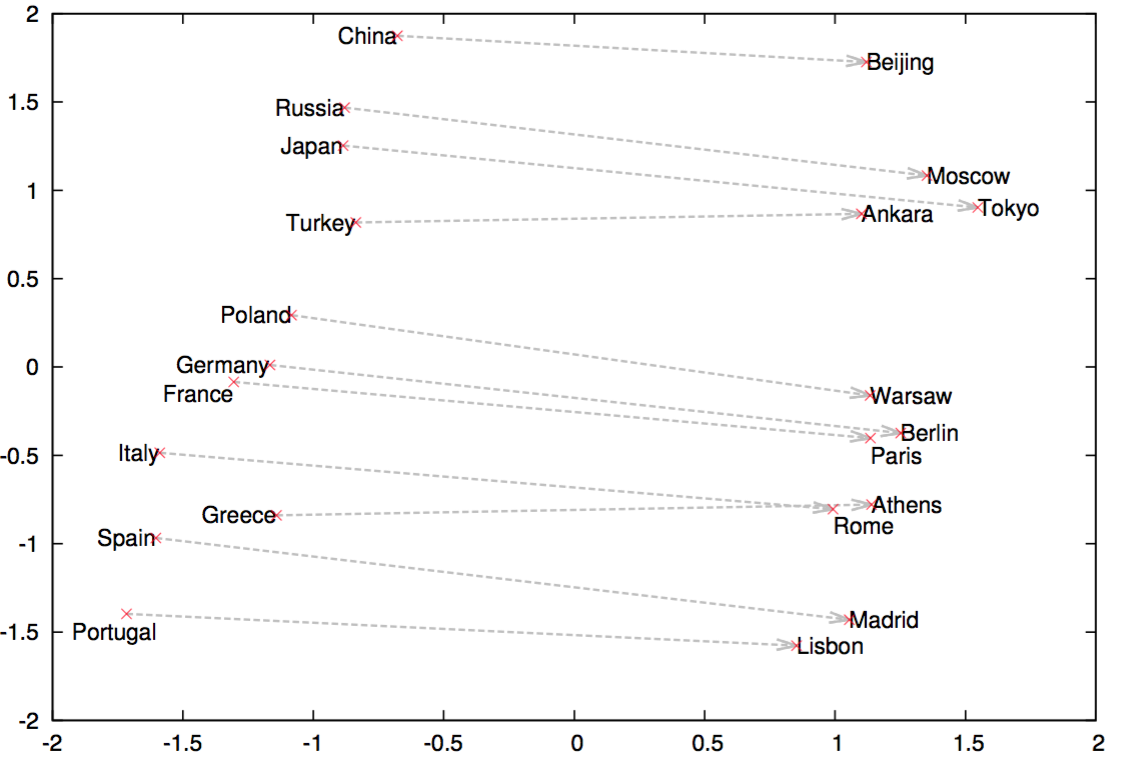
\includegraphics[width=0.8\textwidth]{../img/capitals.png}
    \caption[Hauptstadtrelationen zwischen Wortkontextvektoren]{Hauptstadtrelationen
    zwischen Wortvektoren aus (\cite{mikolov2013distributed}). Die 1000-dimensionalen Vektoren wurden mithilfe von PCA
    auf zwei Dimension projiziert.}\label{fig:capitals}
\end{figure}

Dies könnte man dann insofern ausnutzen, indem man ein Clusteringverfahren anwendet, um Gruppen mit ähnlichen
Differenzvektoren zu identifizieren und die Elemente jeder Gruppe danach mit der entsprechenden Relation in einen
Wissensgraphen einzuordnen. Dies hätte zwei Vorteile:
\begin{enumerate}
  \item Teile des kostenintensiven Dateneinpflegens durch menschliche Hilfe fällt weg
  \item Es wird ersichtlich, welche semantischen Relationen in einem Raum von Wortkontextvektoren tatsächlich abgebildet
  werden klnnen.
\end{enumerate}

Die Ergebnisse, die diese Prozedur und andere Experimente zutage fördern sowie die Fallstricke, die diese mit sich
bringen, werden in den nächsten Kapiteln beschrieben. Über jene wird nun ein kleiner Überblick gegeben.

\section{Inhalt}

In Kapitel \ref{Chapter2} dieser Arbeit sollen verwandte Werke zu den erwähnten Themen referenziert werden.
Daraufhin folgt in Kapitel \ref{Chapter3} die Darlegung einiger für das Verständnis essenzieller Grundlagen, wie z.B.
neurale Netze und ihre Nutzung zum Erstellen von Wortkontextvektoren.\\
Die in Kapitel \ref{Chapter4} beschriebenen Vorbereitungsschritte und eine ausführliche Evaluation von Wortkontextvektoren
\ref{Chapter5} leiten auf die drei Experimente in den Kapiteln \ref{Chapter6}, \ref{Chapter7} und \ref{Chapter8} über:
\begin{itemize}
  \item[$\mathcal{A}$:] Reproduktion des Ansatzes von (\cite{bordes2013translating}) mit einem kleineren Datenset
  \item[$\mathcal{B}$:] Indentifikation von Wortpaaren gleicher Relation durch Clustering
  \item[$\mathcal{C}$:] Training von Relationsrepräsentationen ähnlich (\cite{bordes2013translating}) mit Wortkontextvektoren
\end{itemize}

Zuletzt folgt ein Gesamtfazit der Arbeit mit Ausblick (siehe Kapitel \ref{Chapter9}) mit zwei Appendices \ref{AppendixA}
und \ref{AppendixB} mit detaillierten Informationen über Wortkontextvektortraining und -evaluation sowie die
\ref{sec:bib}.
